\section{Introduction}

%\paragraph{Background and Challenges}
Action recognition in videos has been one of the active research fields in computer vision \cite{pirsiavash2012detecting, poppe2010survey} due to its wide applications in areas like surveillance, video retrieval, human-computer interaction and smart environments.
Because of the diversity and complexity of actions, and complicated environment (e.g background clutter and illumination variation), action recognition is still a challenging problem.
In order to solve this problem, related approaches can be divided into three major directions, including silhouette-based \cite{blank2005actions, ke2007event, vitaladevuni2008action, yilmaz2005actions}, salient point-based \cite{laptev2005space, dollar2005behavior, laptev2008learning, bregonzio2009recognising, klaser2008aspatiotemporal, willems2008efficient} and trajectory-based \cite{matikainen2009trajectons, messing2009activity, sun2009hierarchical}.
All the three approaches, especially, try to capture motion information that appears in videos, since motion is crucial information for presenting actions.
Based on work of H.Wang et al. \cite{wang2011densetraj}, dense trajectory-based approach has been demonstrated that it is the state-of-the-art approach for action recognition.
Recently, the dense trajectory-based motion feature proposed by \cite{wang2011densetraj} has achieved the state-of-the-art performances on multimedia event detection (MED) systems, such as, segment-based system \cite{phan2014multimedia} on TRECVID MED 2010, 2011, or AXES \cite{oneata2012axes}, and BBNVISER \cite{natarajan2012bbn} on TRECVID MED 2012.

%\paragraph{Existing approaches and drawbacks}
In the past decades, most studies in human action recognition mainly investigate on video sequences captured by traditional 2D cameras.
Although, there are many advanced approaches for action recognition in domain of 2D videos, the mentioned challenges are still difficult to handle.
With the development of new RGB-D cameras, e.g. Kinect camera, capturing color images as well as depth maps has become feasible in real time.
The depth maps can enrich information for cues, such as body shape and motion information to discriminate actions.
In addition, challenges appeared in RGB data such as illumination variations and background clutter can be dealt with by depth data.
Due to these advantages, recent research trend concentrates on exploiting depth maps for action recognition \cite{li2010action, wang2012mining, vieira2012stop, yang2012eigenjoints, yang2012recognizing, wang2012robust, xia2013spatio, oreifej2013hon4d}.
Works \cite{li2010action, yang2012recognizing, xia2013spatio} leverage the 2D technique robustness to adapt for depth video.
In contrast, others \cite{vieira2012stop, wang2012robust, oreifej2013hon4d} propose methods to recognize actions in depth videos as in 4D data.
Besides, skeleton information, the higher-level information of depth data, is also proposed to use in works \cite{wang2012mining, yang2012eigenjoints}.
However, in our best knowledge, none success with combining dense trajectories, the state-of-the-art approach on 2D video, and depth video.
In this paper, we investigate to exploit the dense trajectory-based approach on depth video.

%\paragraph{Proposal, Idea and Steps}
The dense trajectory-based approach leverages dense sampling to keep most discriminative trajectories in video.
Therefore, in order to effectively exploit this approach on depth video, it is necessary to exactly extract discriminative trajectories in depth video.
To perform this requirement, a straightforward method is to consider depth value as intensity value and adapts extracting dense trajectories on 2D transformed video.
However, this way can cause confused cases of action classes.
For example, \textit{forward punch} and \textit{hammer} may be confused actions, if we view them from front, since they contain similar movements respectively: “lift arm up” and “stretch out”.
Therefore the additional information is needed to distinguish such actions.

\begin{figure}[H]
	\begin{center}
		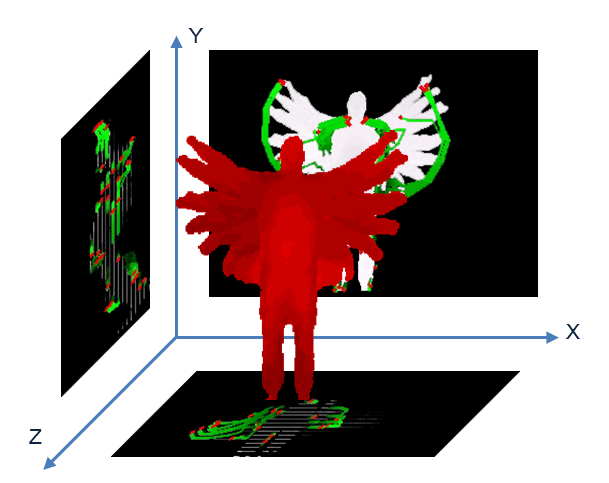
\includegraphics[width=0.7\textwidth]{Projections.png}
	\end{center}
	\caption{\label{lbl:Figure_ProposedMethod}Illustration of our trajectory-based approach. The original sequence of depth maps is projected onto three orthogonal planes to form intensity videos. After that, the dense trajectory motion features are calculated for each representation.}
\end{figure}

The basis idea to deal with such cases is to watch actions from various views.
Information achieved from the views can provide clearer cues to discriminate such actions.
To collect such information from depth video, a simple way is to project depth maps onto view planes, see figure \ref{lbl:Figure_ProposedMethod}.
The projections are easily obtained by the mentioned advantages of depth data.
Data projected on the planes is then gathered to generate corresponding 2D videos.
Dense trajectory-based motion features are then calculated on 2D videos to generate a final feature representation for depth video.

%\paragraph{Experiments and Results}
To evaluate the effectiveness of our method, we conduct experiments on MSR Action 3D dataset and MSR Daily Activity 3D dataset.
Experimental results show that our proposed method beats the state-of-the-art methods in constrain of only using depth data.
The results also present our contributions: (1) we propose an effective method to exploit trajectories in depth video, (2) we perform comprehensive experiments on the challenging benchmark dataset and indicate that our proposed method is the best when compared with the state-of-the-art depth-based methods.

%\paragraph{Paper structure}
After a brief review of the related work in Section \ref{lbl:RelatedWorks}, the proposed method is described in Section \ref{lbl:ProposedMethod}. Sections \ref{lbl:ExperimentalSettings} and \ref{lbl:ExperimentalResults} present the experimental settings and results. In section \ref{lbl:Discussions} we provide some concerned discussions. The summaries of our work are given in Section \ref{lbl:Conclusions}.
